% file: 3-8-apsp/undirected-graph.tex

\documentclass[tikz]{standalone}
\usetikzlibrary{positioning}

\begin{document}
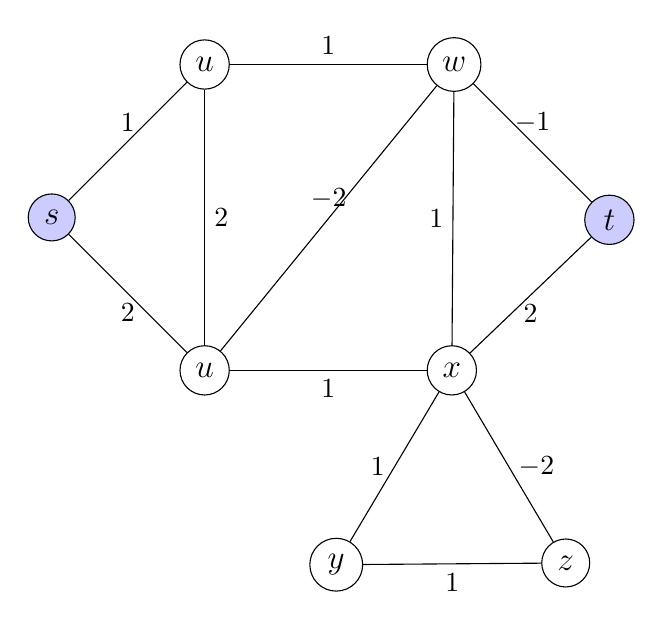
\begin{tikzpicture}[vertex/.style = {draw, circle, minimum size = 8pt, font = \large},
    node distance = 1.5 and 1.5cm,
    every edge/.style = {draw, -}]

  \node (s) [fill = blue!20, vertex] {$s$};
  \node (u) [vertex, above right = of s] {$u$};
  \node (v) [vertex, below right = of s] {$u$};

  \node (w) [vertex, right = 2.5cm of u] {$w$};
  \node (t) [fill = blue!20, vertex, below right = of w] {$t$};

  \node (x) [vertex, right = 2.5cm of v] {$x$};
  \node (y) [vertex, below left = 2.0cm and 1.0cm of x] {$y$};
  \node (z) [vertex, below right = 2.0cm and 1.0cm of x] {$z$};

  \path (s) edge node [above] {$1$} (u)
	(u) edge node [above] {$1$} (w)
	    edge node [right] {$2$} (v)
	(w) edge node [above] {$-1$} (t)
	    edge node [above] {$-2$} (v)
	    edge node [left] {$1$} (x)
	(t) edge node [below] {$2$} (x)
	(x) edge node [below] {$1$} (v)
	    edge node [left] {$1$} (y)
	    edge node [right] {$-2$} (z)
	(y) edge node [below] {$1$} (z)
	(v) edge node [below] {$2$} (s);
\end{tikzpicture}
\end{document}
